\documentclass[14pt]{extbook}
\usepackage{multicol, enumerate, enumitem, hyperref, color, soul, setspace, parskip, fancyhdr} %General Packages
\usepackage{amssymb, amsthm, amsmath, latexsym, units, mathtools} %Math Packages
\everymath{\displaystyle} %All math in Display Style
% Packages with additional options
\usepackage[headsep=0.5cm,headheight=12pt, left=1 in,right= 1 in,top= 1 in,bottom= 1 in]{geometry}
\usepackage[usenames,dvipsnames]{xcolor}
\usepackage{dashrule}  % Package to use the command below to create lines between items
\newcommand{\litem}[1]{\item#1\hspace*{-1cm}\rule{\textwidth}{0.4pt}}
\pagestyle{fancy}
\lhead{Progress Quiz 10}
\chead{}
\rhead{Version B}
\lfoot{5170-5105}
\cfoot{}
\rfoot{Summer C 2021}
\begin{document}

\begin{enumerate}
\litem{
Choose the equation of the function graphed below.
\begin{center}
    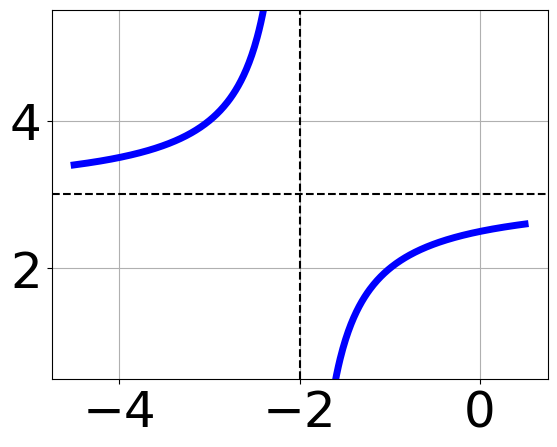
\includegraphics[width=0.5\textwidth]{../Figures/rationalGraphToEquationCopyB.png}
\end{center}
\begin{enumerate}[label=\Alph*.]
\item \( f(x) = \frac{-1}{x + 2} + 3 \)
\item \( f(x) = \frac{1}{(x - 2)^2} + 3 \)
\item \( f(x) = \frac{-1}{(x + 2)^2} + 3 \)
\item \( f(x) = \frac{1}{x - 2} + 3 \)
\item \( \text{None of the above} \)

\end{enumerate} }
\litem{
Solve the rational equation below. Then, choose the interval(s) that the solution(s) belongs to.\[ \frac{-84}{84x + 36} + 1 = \frac{-84}{84x + 36} \]\begin{enumerate}[label=\Alph*.]
\item \( x \in [-1.43,0.57] \)
\item \( x \in [0,1.3] \)
\item \( x_1 \in [-0.7, 0.2] \text{ and } x_2 \in [-0.4,1.7] \)
\item \( x_1 \in [-0.7, 0.2] \text{ and } x_2 \in [-0.9,-0.2] \)
\item \( \text{All solutions lead to invalid or complex values in the equation.} \)

\end{enumerate} }
\litem{
Determine the domain of the function below.\[ f(x) = \frac{6}{25x^{2} +45 x + 18} \]\begin{enumerate}[label=\Alph*.]
\item \( \text{All Real numbers except } x = a \text{ and } x = b, \text{ where } a \in [-2.1, -0.7] \text{ and } b \in [-0.9, -0.2] \)
\item \( \text{All Real numbers except } x = a, \text{ where } a \in [-30.6, -29.5] \)
\item \( \text{All Real numbers except } x = a \text{ and } x = b, \text{ where } a \in [-30.6, -29.5] \text{ and } b \in [-15.9, -14.6] \)
\item \( \text{All Real numbers.} \)
\item \( \text{All Real numbers except } x = a, \text{ where } a \in [-2.1, -0.7] \)

\end{enumerate} }
\litem{
Choose the graph of the equation below.\[ f(x) = \frac{1}{(x + 3)^2} - 1 \]\begin{enumerate}[label=\Alph*.]
\begin{multicols}{2}\item 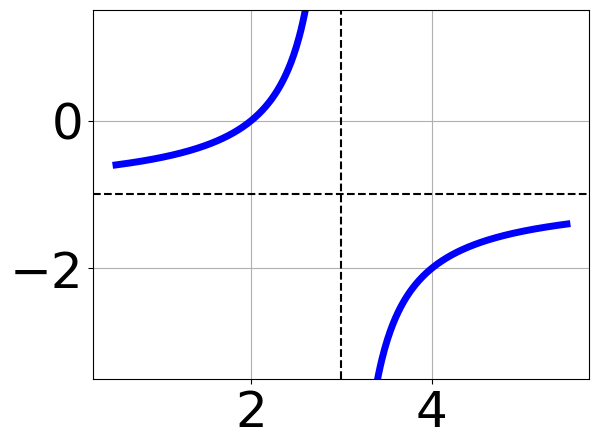
\includegraphics[width = 0.3\textwidth]{../Figures/rationalEquationToGraphCopyAB.png}\item 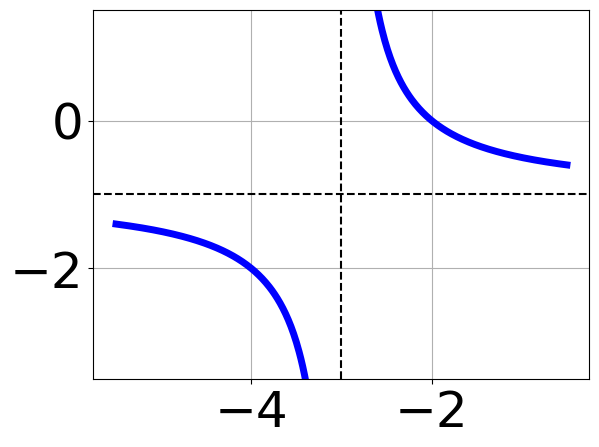
\includegraphics[width = 0.3\textwidth]{../Figures/rationalEquationToGraphCopyBB.png}\item 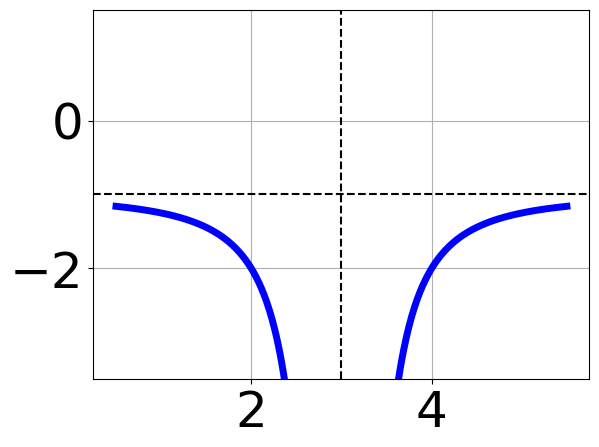
\includegraphics[width = 0.3\textwidth]{../Figures/rationalEquationToGraphCopyCB.png}\item 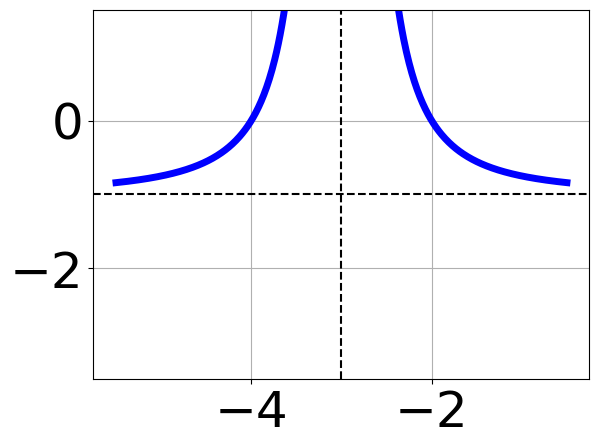
\includegraphics[width = 0.3\textwidth]{../Figures/rationalEquationToGraphCopyDB.png}\end{multicols}\item None of the above.
\end{enumerate} }
\litem{
Solve the rational equation below. Then, choose the interval(s) that the solution(s) belongs to.\[ \frac{-6x}{-7x -5} + \frac{-3x^{2}}{-14x^{2} -38 x -20} = \frac{-5}{2x + 4} \]\begin{enumerate}[label=\Alph*.]
\item \( \text{All solutions lead to invalid or complex values in the equation.} \)
\item \( x_1 \in [-3.93, -2.1] \text{ and } x_2 \in [-1.07,-0.51] \)
\item \( x \in [-2.81,-0.99] \)
\item \( x_1 \in [-3.93, -2.1] \text{ and } x_2 \in [-0.69,-0.27] \)
\item \( x \in [-0.99,0.12] \)

\end{enumerate} }
\litem{
Choose the equation of the function graphed below.
\begin{center}
    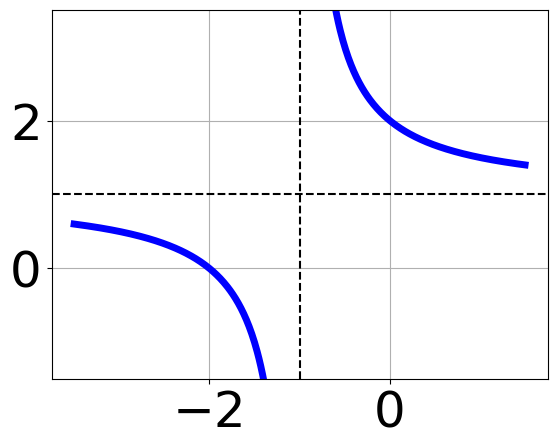
\includegraphics[width=0.5\textwidth]{../Figures/rationalGraphToEquationB.png}
\end{center}
\begin{enumerate}[label=\Alph*.]
\item \( f(x) = \frac{-1}{x - 1} + 1 \)
\item \( f(x) = \frac{1}{x + 1} + 1 \)
\item \( f(x) = \frac{-1}{(x - 1)^2} + 1 \)
\item \( f(x) = \frac{1}{(x + 1)^2} + 1 \)
\item \( \text{None of the above} \)

\end{enumerate} }
\litem{
Determine the domain of the function below.\[ f(x) = \frac{4}{15x^{2} +24 x + 9} \]\begin{enumerate}[label=\Alph*.]
\item \( \text{All Real numbers.} \)
\item \( \text{All Real numbers except } x = a, \text{ where } a \in [-15.49, -14.95] \)
\item \( \text{All Real numbers except } x = a \text{ and } x = b, \text{ where } a \in [-15.49, -14.95] \text{ and } b \in [-9.13, -8.74] \)
\item \( \text{All Real numbers except } x = a \text{ and } x = b, \text{ where } a \in [-1.44, -0.83] \text{ and } b \in [-0.78, -0.34] \)
\item \( \text{All Real numbers except } x = a, \text{ where } a \in [-1.44, -0.83] \)

\end{enumerate} }
\litem{
Choose the graph of the equation below.\[ f(x) = \frac{1}{(x + 3)^2} + 3 \]\begin{enumerate}[label=\Alph*.]
\begin{multicols}{2}\item 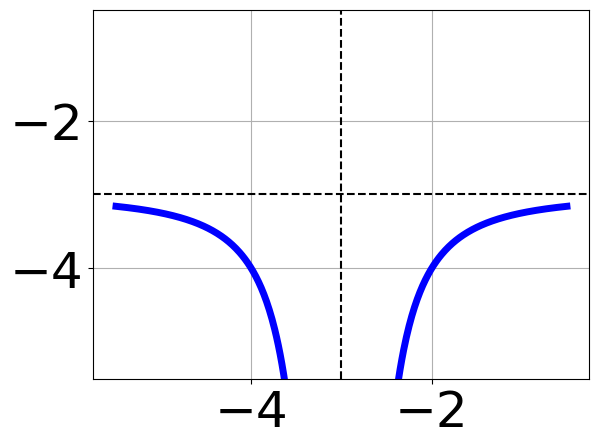
\includegraphics[width = 0.3\textwidth]{../Figures/rationalEquationToGraphAB.png}\item 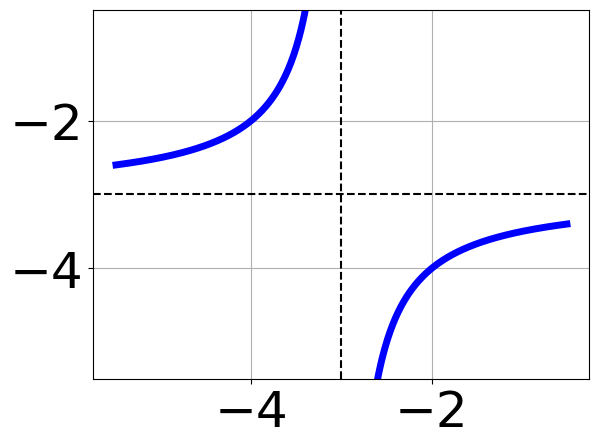
\includegraphics[width = 0.3\textwidth]{../Figures/rationalEquationToGraphBB.png}\item 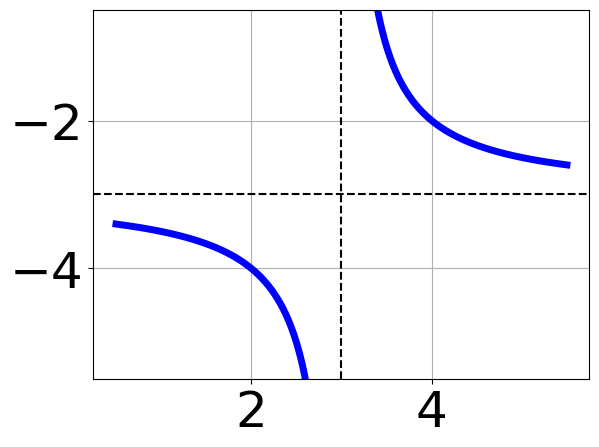
\includegraphics[width = 0.3\textwidth]{../Figures/rationalEquationToGraphCB.png}\item 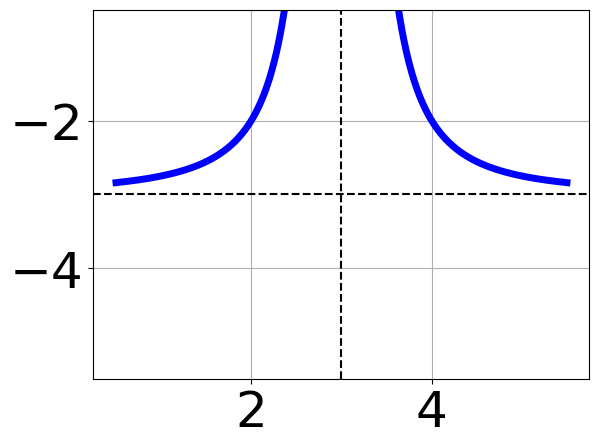
\includegraphics[width = 0.3\textwidth]{../Figures/rationalEquationToGraphDB.png}\end{multicols}\item None of the above.
\end{enumerate} }
\litem{
Solve the rational equation below. Then, choose the interval(s) that the solution(s) belongs to.\[ \frac{-5x}{4x + 3} + \frac{-2x^{2}}{-12x^{2} +19 x + 21} = \frac{-7}{-3x + 7} \]\begin{enumerate}[label=\Alph*.]
\item \( \text{All solutions lead to invalid or complex values in the equation.} \)
\item \( x \in [2.32,2.42] \)
\item \( x \in [-0.88,-0.65] \)
\item \( x_1 \in [-0.97, -0.81] \text{ and } x_2 \in [0.47,1.31] \)
\item \( x_1 \in [-0.88, -0.65] \text{ and } x_2 \in [2.07,3.03] \)

\end{enumerate} }
\litem{
Solve the rational equation below. Then, choose the interval(s) that the solution(s) belongs to.\[ \frac{-24}{60x -24} + 1 = \frac{-24}{60x -24} \]\begin{enumerate}[label=\Alph*.]
\item \( x_1 \in [-0.5, -0.2] \text{ and } x_2 \in [0.4,2.4] \)
\item \( x_1 \in [0.3, 0.8] \text{ and } x_2 \in [0.4,2.4] \)
\item \( x \in [0.4,1.4] \)
\item \( \text{All solutions lead to invalid or complex values in the equation.} \)
\item \( x \in [-0.5,-0.2] \)

\end{enumerate} }
\end{enumerate}

\end{document}